% Homework 5 - CS386(late submission)
% Russell Miller Winter 2011

\documentclass{article}
\usepackage{anysize}
\usepackage{wasysym}
\usepackage{graphicx}

\marginsize{2cm}{2cm}{2cm}{2cm}

\title{CS386 Homework 5}
\author{Russell Miller}
\date{\today}

\begin{document}

\maketitle

\section{}
\begin{description}
\item[a.]
ERD with cardinality constraints:\footnotemark\\
\footnotetext{ERDs drawn using Dia. http://projects.gnome.org/dia/\\
Edited with the GIMP [GNU Image Manipulation Program]}
\begin{center}
 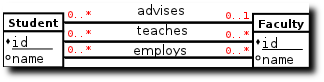
\includegraphics[scale=.8]{1a.png}
\end{center}
Relational Schema for this ERD:
\begin{quote}
\textbf{Student}(\underline{id}, name, advisor) advisor references Faculty.id\\
\textbf{Faculty}(\underline{id}, name)\\
\textbf{Teachers}(\underline{faculty\_id, student\_id}) faculty\_id references Faculty.id, student\_id 
references Student.id\\
\textbf{Employments}(\underline{faculty\_id, student\_id}) faculty\_id references Faculty.id, student\_id 
references Student.id\\
\end{quote}

\item[b.]
ERD with cardinality contraints:\\
\begin{center}
 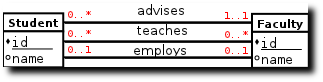
\includegraphics[scale=.8]{1b.png}
\end{center}
Relational Schema:
\begin{quote}
\textbf{Student}(\underline{id}, name, advisor, employer) advisor not null and references Faculty.id, employer references Faculty.id\\
\textbf{Faculty}(\underline{id}, name, employee) employee references Student.id\\
\textbf{Teachings}(\underline{faculty\_id, student\_id}) faculty\_id references Faculty.id, student\_id
references Student.id\\
\end{quote}
\end{description}

\section{}
\textbf{Person\\}
\begin{description}
\item[a.]
$\quad id \rightarrow ssn,name,phone$\\
$ssn \rightarrow name$
\item[b.]
$\quad id,ssn \rightarrow id$\\
$id,ssn \rightarrow ssn$\\
$id,name \rightarrow name$\\
$id,phone \rightarrow phone$
\item[c.]
$\quad none$
\item[d.]
$\quad none$
\item[e.]
$\quad none$
\end{description}

\end{document}
